\documentclass[11pt]{amsart}
\usepackage[marginratio=1:1, headheight=27pt,
footskip = 13pt, a4paper, total={6.5in, 8in}]{geometry}                % See geometry.pdf to learn the layout options. There are lots.
\geometry{letterpaper}                   % ... or a4paper or a5paper or ...
%\geometry{landscape}                % Activate for for rotated page geometry
%\usepackage[parfill]{parskip}    % Activate to begin paragraphs with an empty line rather than an indent
\usepackage{graphicx}
\usepackage[font=small,labelfont=bf]{caption} % Required for specifying captions to tables
\usepackage{dirtytalk}
%\usepackage[version=3]{mhchem}
%\usepackage{subcaption}
\usepackage{subfig}
%\usepackage{epstopdf}
\usepackage{booktabs}
\usepackage[compact,small]{titlesec}
\usepackage{complexity}
%\usepackage[sc, osf]{mathpazo} % add possibly `sc` and `osf` options
%\usepackage{eulervm}
%\usepackage{textcomp}

\clubpenalty = 10000
\widowpenalty = 10000
%\usepackage[altbullet]{lucidabr}
\usepackage{float}
\usepackage{siunitx}
\usepackage[justification=centering]{caption}
\usepackage[
colorlinks = true,
urlcolor = blue
]{hyperref}
\usepackage{mathrsfs}
\usepackage{amssymb}
\usepackage{mathtools}
\usepackage{amsmath}
\usepackage{amsthm}
\renewcommand\qedsymbol{$\blacksquare$}

\usepackage[section]{placeins}
\DeclareGraphicsRule{.tif}{png}{.png}{`convert #1 `dirname #1`/`basename #1 .tif`.png}

%\usepackage[swedish]{babel}
\usepackage[T1]{fontenc}
\usepackage[utf8]{inputenc}

\usepackage{comment}
\usepackage{enumitem}
\titleformat{\section}[block]{\large\scshape\centering}{\thesection.}{1em}{}
\titleformat{\subsection}[block]{\large}{\thesubsection.}{1em}{}

\usepackage{pgfplots}
\pgfplotsset{compat = 1.15}

\usepackage{listings}
\lstset{basicstyle=\ttfamily,breaklines=true}
\usepackage{color} %red, green, blue, yellow, cyan, magenta, black, white
\definecolor{mygreen}{RGB}{28,172,0} % color values Red, Green, Blue
\definecolor{mylilas}{RGB}{170,55,241}

%\usepackage{times}
%\usepackage{kpfonts}
%\usepackage{txfonts}
%\usepackage{newtx}
%\usepackage{stix}
%\usepackage[osf,proportional]{libertine}
%\usepackage{lmodern}
\usepackage[charter]{mathdesign}

\usepackage{microtype}
%\usepackage{stix}
\usepackage[compact,small]{titlesec}
\titleformat*{\section}{\large\bfseries\sffamily}

\titleformat*{\subsection}{\small\bfseries\sffamily}
\titleformat*{\subsubsection}{\small\bfseries\sffamily}
%\renewcommand{\section}{\section*}
\newcommand{\ibits}{\{0, 1\}^*}
%\renewcommand{\familydefault}{\sfdefault}
\usepackage{marginnote}
\renewcommand*{\marginfont}{\color{red}\sffamily\footnotesize}
\usepackage{hyperref, xcolor}

%\usepackage{makeidx}
\definecolor{winered}{rgb}{0.5,0,0}
\hypersetup{
     pdfauthor={JAG},
     pdfsubject={Hyperlinks in LaTeX},
     pdftitle={main.tex},
     pdfkeywords={LaTeX, PDF, hyperlinks}
%    colorlinks=false,
     pdfborder={0 0 0},
%You can set individual colors for links as below:
colorlinks=true,
  linkcolor=winered,
urlcolor={winered},
filecolor={winered},
citecolor={winered},
allcolors={winered}
}

\usepackage[english]{babel} 
\usepackage[
backend=biber,
style=numeric,
hyperref=true,
%natbib
]{biblatex}
\DeclareLanguageMapping{swedish}{swedish-apa}
\addbibresource{Komplexitetsteori.bib}

\usepackage[T1]{fontenc}

%\usepackage{fouriernc}

\usepackage{thmtools}
\usepackage{fancyhdr}
\usepackage{csquotes}
\newsavebox{\myheadbox}
\fancypagestyle{normalpage}
{
%\begin{flushright}
\lhead{
Jonas Conneryd
}
%\end{flushright}
\rhead{\url{conneryd@kth.se}}
\chead{MM8042 Algebraic Topology}
\cfoot{\thepage}
}
\fancyhf{}
\fancypagestyle{firstpage}
{
%\begin{flushright}
\lhead{
Jonas Conneryd \\ \url{conneryd@kth.se}}
%\end{flushright}
\rhead{970731-7559  \\
\the\year
}
\chead{\Large{\scshape{\textbf{Homework 1} \\ \vspace{-4pt}\normalsize\textbf{ MM8042 Algebraic Topology}}}}
\cfoot{\thepage}
}

\pagestyle{normalpage}

\declaretheoremstyle[headfont=\bfseries\sffamily]{normalhead}
\interfootnotelinepenalty=10000
%\title{\vspace{-2cm}\textbf{\textsf{ Homework 3}}}
\date{}
%\author{Jonas Conneryd \\
%conneryd@kth.se \\ 970731-7559}

\newcommand{\Set}{\mathsf{Set}}
\renewcommand{\C}{\mathsf{C}}
\begin{document}
%\maketitle
\thispagestyle{firstpage}
\theoremstyle{normalhead}
\newtheorem{problem}{Problem}
\newtheorem{lemma}{Lemma}

\begin{problem}
\textbf{(W)} Suppose that $X_\bullet$ is a finite $\Delta$-complex. Define the \emph{Euler characteristic} of $X_\bullet$ to be the alternating sum $\chi(X_\bullet) = \# X_0-\#X_1+\#X_2-\ldots$. Though it is not obvious from the definition, one can show that all different $\Delta$-structures on the same space will have the same Euler characteristic. Find two different $\Delta$-structures on the torus and verify that they give the same Euler characteristic.
\end{problem}

\begin{proof}[Solution]
Consider the following $\Delta$-structures on the torus:
\begin{center}
    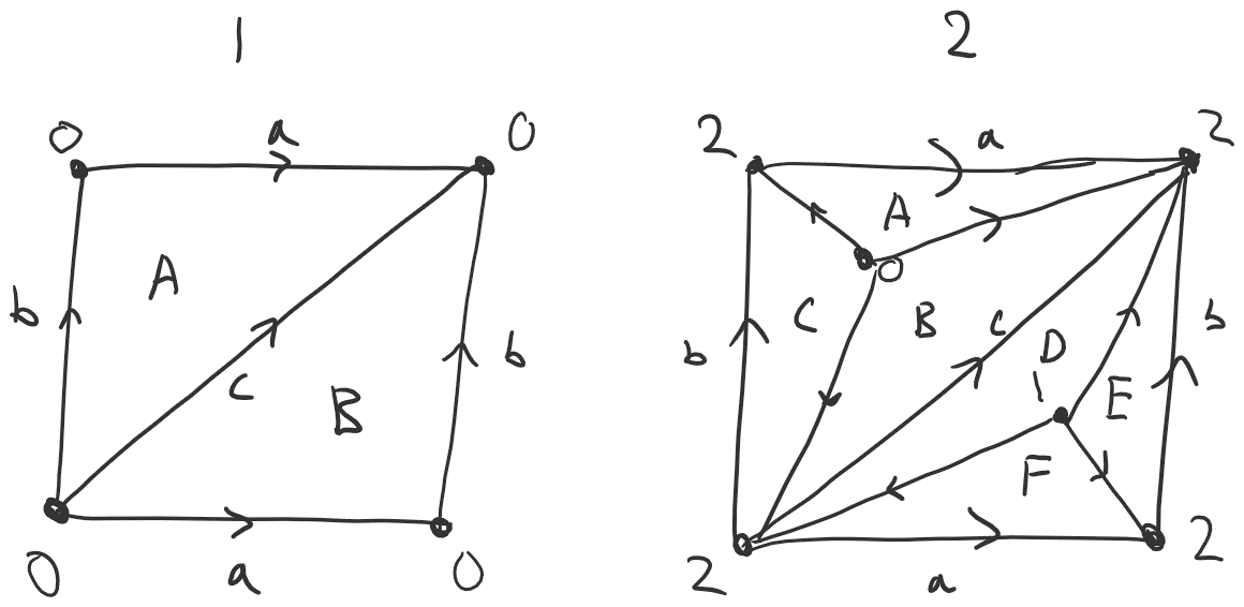
\includegraphics[width = 0.7\textwidth]{Picture1.png}.
\end{center}
In \textbf{1}, we have one 0-simplex (0), three 1-simplices ($a, b, c$) and two 2-simplices ($A, B$). The Euler characteristic is therefore $1-3+2=0$. In \textbf{2}, we have three 0-simplices (0, 1, 2), nine 1-simplices($a, b, c$ and the other, unidentified, 1-simplices), and six $2$-simplices ($A, B, C, D, E, F$). The Euler characteristic is therefore $3-9+6 = 0$. 
\end{proof}

\newpage


\begin{problem}
\textbf{(W)} Let $\mathsf{C}$ be a category, and let $\alpha: x\to y$ be a morphism in $\C$. We say that $\alpha$ is an \emph{isomorphism} if there exists another morphism $\beta: y \to x$ such that $\alpha \circ \beta = \mathsf{1}_y$ and $\beta \circ  \alpha  = \mathsf{1}_x$.
\begin{enumerate}[font=\normalfont,label=\textbf{(\alph*)}]
\item Prove that if such $\beta$ exists, it is unique. We will therefore write $\alpha^{-1}$ for this morphism. 

\item Let $\mathsf{Aut}(x)$ be the set of all isomorphisms of $x$ with itself. Prove that $\mathsf{Aut}(x)$ is a group.

\item Prove that if there is an isomorphism of objects $x$ and $y$ then there is an isomorphism of groups  $\mathsf{Aut}(x) \cong \mathsf{Aut}(y)$. 
\end{enumerate}
\end{problem}

\begin{proof}[Solution]
\hfill
\begin{enumerate}[font=\normalfont,label=\textbf{(\alph*)}, wide]
\item Let $\alpha: x\to y$ be a morphism, and suppose there are two maps $\beta_1, \beta_2: y \to x$ that make $\alpha$ into an isomorphism. Then we have
\[
\begin{aligned}
\alpha \circ \beta_1 &= \alpha \circ \beta_2 = 1_y, \\
 \beta_1  \circ \alpha&= \beta_2 \circ \alpha  = 1_x.
\end{aligned}
\]
This implies that
\[
\begin{aligned}
\beta_2 \circ ( \alpha \circ \beta_1) &= \beta_2 \circ ( \alpha \circ \beta_2) = \beta_2 \circ 1_y, \\
(\beta_1  \circ \alpha) \circ \beta_2 &= (\beta_2 \circ \alpha) \circ \beta_2  = 1_x \circ \beta_2.
\end{aligned}
\]
By associativity of morphism composition (which is guaranteed by the definition of a morphism) and using that $\beta_i \circ 1_y = 1_x \circ \beta_i = \beta_i$, we get
\[
\beta_2 = \beta_2 \circ( \alpha \circ \beta_1) =  (\beta_2 \circ \alpha) \circ \beta_1 = \beta_1, 
\]
so $\beta$ is unique.

\item We need to check closure, identity, inverse and associativity. An identity element for $\mathsf{Aut}(x)$ is provided by $1_x$, which is an isomorphism with inverse $1_x$. Associativity is provided by associativity of morphism composition, which holds by definition. An inverse for the isomorphism $\alpha: x \to x$ is provided by $\beta: x \to x$, where $\beta$ is as in the definition of isomorphism in the problem formulation. $\beta$ is itself an isomorphism with inverse $\alpha$, so it is in $\mathsf{Aut}(x)$. Finally, closure holds because for isomorphisms $\alpha_1, \alpha_2$ with inverses $\beta_1, \beta_2$ respectively, the composed map $\alpha_1 \circ \alpha_2$ is an isomorphism with inverse $\beta_2 \circ \beta_1$, where we have again invoked associativity of morphism composition.


\item Suppose we have an isomorphism $\alpha: x \to y$ with inverse $\alpha: y \to x$. Define $\phi: \mathsf{Aut}(x) \to \mathsf{Aut}(y); g_x \to \alpha \circ g_x \circ \alpha^{-1}$. $\phi(g_x)$ is a morphism $\phi(g_x): y\to y$ with inverse $\alpha \circ g_x^{-1} \circ \alpha^{-1} : y \to y$, so $\phi(g_x)$ is an isomorphism. Clearly, $\phi$ is well-defined. $\phi$ is a homomorphism since 
\[
\begin{aligned}
\phi(g_{x_1}\circ g_{x_2}) &= \alpha \circ g_{x_1}\circ g_{x_2} \circ \alpha^{-1} \\
&= \alpha \circ g_{x_1} \circ \text{Id}_x \circ g_{x_2} \circ \alpha^{-1} \\
&= \alpha \circ g_{x_1} \circ \alpha^{-1} \circ \alpha \circ g_{x_2} \circ \alpha^{-1} \\
&= \phi(g_{x_1})\circ \phi(g_{x_2}).
\end{aligned}
\]
Moreover, $\phi$ is surjective since an arbitrary morphism $g_y \in \mathsf{Aut}(y)$ can be written as $\phi(\alpha^{-1} \circ g_y \circ \alpha)$, where $\alpha^{-1} \circ g_y \circ \alpha \in \mathsf{Aut}(x)$ by arguments analogous to the above. Finally, $\phi$ is injective since an inverse $\phi^{-1}: \mathsf{Aut}(y) \to \mathsf{Aut}(x)$ is furnished by $\phi^{-1}(g_y) = \alpha^{-1} \circ g_y \circ \alpha$. Hence we have an isomorphism $\mathsf{Aut}(x) \cong \mathsf{Aut}(y)$. 
\end{enumerate}
\end{proof}




\end{document}